\documentclass{report}

\usepackage{graphicx}

\title{NERS 570 Group Project: Thick Origami Kinematics Simulator}
\author{Jacob Pavelka}

\begin{document}
\maketitle
\section*{Introduction}
Kinematic Simulation is an important tool for many problems. For linkage systems, it allows one to study the degrees of freedom of a system or its range of motion.
For structural systems it allows one to study whether or not a system is stable.
For computer graphics, simulating kinematics is important for virtual reality training, video games, rapid digital prototyping, and robotics simulation\cite{SiggraphContact22}.

For our project, we want to develop a kinematic simulator for thick, rigid origami so we can become more familiar with the simulation methods. Understanding the kinematic properties of thick origami is important when it is used in a structural sense.

\section*{Background}
To simulate the kinematics of an object, it first needs a representation in the computer. This is usually done by creating a mesh of the object. There are many methods for creating meshes, but we will use the one described in \cite{zhang2021folding} because it creates a mesh and defines the kinematic constraints simultaneously.

This algorithm begins with a list of nodes that describe the important features of a convex hull. From here, four are chosen randomly such that they creat a tetrahedron, and links are defined between them. Then, another point is chosen randomly and connected to three existing point such that these points form another tetrahedron. Links are created between the three existing nodes and the new node. This process is repeated for all remaining nodes. Figure~\ref{fig:mesh_gen} Illustrates this process.



\begin{figure}[!h]
    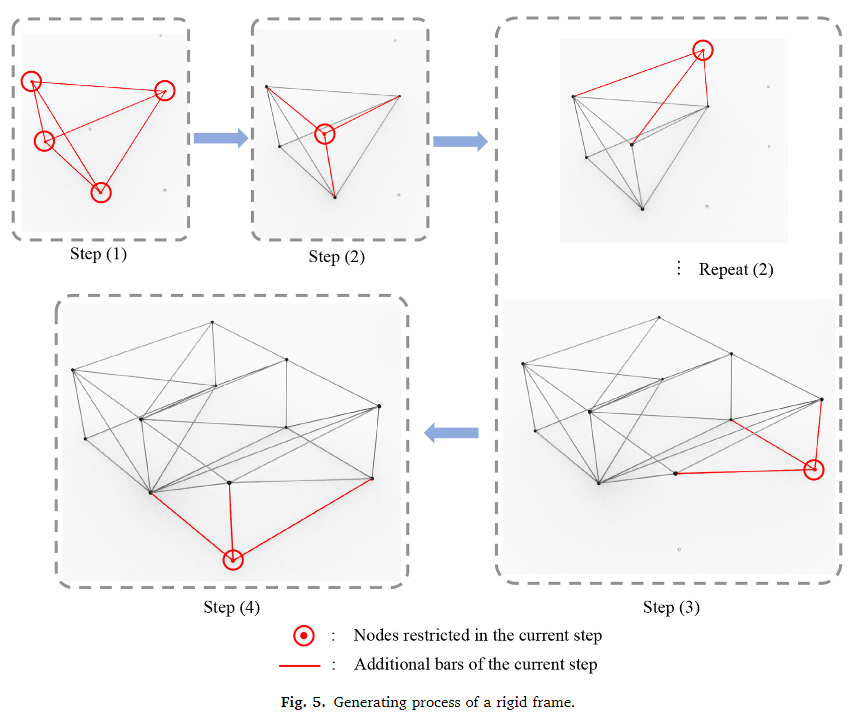
\includegraphics{mesh_gen.png}
\label{fig:mesh_gen}
\end{figure}
\bibliographystyle{plain}
\bibliography{refs}
\end{document}